\lecture{2}{mon 13 sep 9:35}{Economic Systems}
\section{\normalfont Opportunity Cost and the PPC}
\begin{definition}
    A \textbf{Production Possibilities Curve} is an economic model that shows alternative ways that scare resources can be used. The model graphically shows scarcity, trade-offs, and opportunity costs.
\end{definition}
With economic models, there are some assumptions that have to be made for the PPC model to apply,
\begin{itemize}
    \item Only \textbf{TWO} goods can be produced
    \item Full employment of resources
    \item Fixed resources
    \item Fixed technology
\end{itemize}

\begin{figure}[h!]
\begin{center}
\begin{tikzpicture}
\begin{axis}[
scale = 0.9,
xmin = 0, xmax = 10,
ymin = 0, ymax = 10,
axis lines* = left,
xtick = {0}, ytick = \empty,
clip = false,
]
% Production-possibility frontier
\addplot [domain = 0:10, restrict y to domain = 0:10, samples = 10000, color = blue, very thick] {(49-x^2)^0.5};

% Labels
\node [right] at (current axis.right of origin){$A$};
\node [above] at (current axis.above origin) {$B$};
\end{axis}
\end{tikzpicture}
\end{center}
\caption{an example of a PPC curve between good A and good B}
\end{figure}

The data can also be displayed in a \textbf{Production Possibilities Table}, where each point represents a specific combination of goods that can be produced given full employment of resources. 

\begin{table}[h!]
    \begin{center}
      \begin{tabular}{r|c|c|c|c|c}
        \toprule % <-- Toprule here
        \textbf{} & \textbf{A} & \textbf{B} & \textbf{C} & \textbf{D} & \textbf{E}\\
        \midrule % <-- Midrule here
        Bikes & 14 & 12 & 9 & 5 & 0\\
        Computers & 0 & 2 & 4 & 6 & 8\\
        \bottomrule % <-- Bottomrule here
      \end{tabular}
      \caption{Production Possibilties Table between Bikes and Computers}
      \label{tab:table1}
    \end{center}
\end{table}

\begin{figure}[h!]
\begin{center}
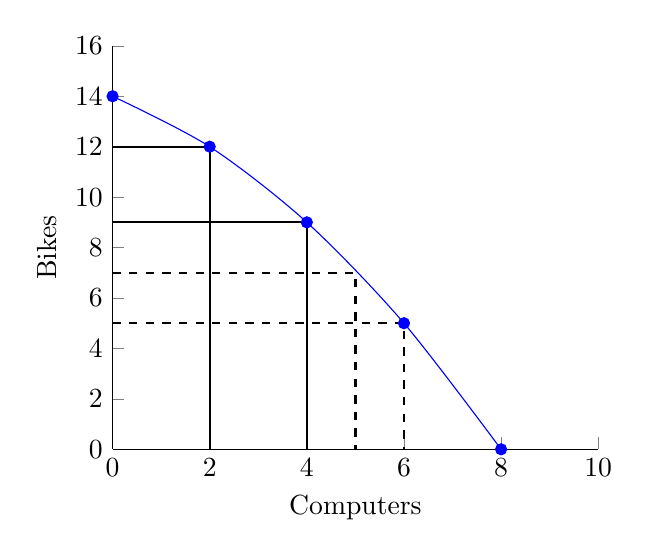
\begin{tikzpicture}
\begin{axis}[
scale = 0.9,
xmin = 0, xmax = 10,
ymin = 0, ymax = 16,
axis lines* = left,
xlabel={Computers},
ylabel={Bikes},
xtick = {0,2,4,6,8,10}, ytick = {0,2,4,6,8,10,12,14,16},
clip = false,
]

\addplot [color = blue,mark=*,mark options={solid},smooth]
    coordinates {
        (0,14)(2,12)(4,9)(6,5)(8,0)
    };

\addplot[color = black, solid, thick] coordinates {(0, 12) (2, 12) (2, 0)};
\addplot[color = black, solid, thick] coordinates {(0, 9) (4, 9) (4, 0)};
\addplot[color = black, dashed, thick] coordinates {(0, 7) (5, 7) (5, 0)};
\addplot[color = black, dashed, thick] coordinates {(0, 5) (6, 5) (6, 0)};

\end{axis}
\end{tikzpicture}
\end{center}
\caption{Graph of Production}
\end{figure}

The table demonstrates how much of each good can be produced with full employment of resources. Country X can produce 14 Bikes or 8 Computers if they solely focus on producing said good. If we take the points and plot them, we get a PPC curve.

The PPC can shift, just like any econonmics graph. Make sure you can logically reason through why 
\begin{example}
    What happens if there is an increase in population?
    \begin{center}
    \begin{tikzpicture}
    \begin{axis}[
    scale = 0.7,
    xmin = 0, xmax = 10,
    ymin = 0, ymax = 10,
    axis lines* = left,
    xtick = {0}, ytick = \empty,
    axis on top,
    clip = false,
    ]
% Production-possibility frontier
    \addplot [domain = 0:10, restrict y to domain = 0:10, samples=10000, color = blue, very thick, name path = frontier]{(30-x^2)^0.5};
    \addplot [domain = 0:10, restrict y to domain = 0:10, draw = none, name path = axis]{0};
    \addplot [domain = 0:10, restrict y to domain = 0:10, samples=10000, color = blue, very thick, name path = increase]{(60-x^2)^0.5};

    % Colouring areas
    \addplot [blue,  opacity = 0.1] fill between [of = frontier and axis];
    \addplot [blue, opacity = 0.2] fill between [of = increase and frontier];

    % Arrow
    \draw[-{Triangle[length=2mm, width=1mm]}, black,] (6, 2) to (7, 2);
    % Labels
    \node [right] at (current axis.right of origin) {$A$};
    \node [above] at (current axis.above origin) {$B$};
    \end{axis}
    \end{tikzpicture}
    \end{center}
\end{example}
\begin{example}
    What happens when Good A technology improves
    \begin{center}
    \begin{tikzpicture}
    \begin{axis}[
      scale = 0.7,
      xmin = 0, xmax = 10,
      ymin = 0, ymax = 10,
      axis lines* = left,
      xtick = {0}, ytick = \empty,
      axis on top,
      clip = false,
      ]
  % Production-possibility frontier
      \addplot [domain = 0:10, restrict y to domain = 0:10, samples=10000, color = blue, very thick, name path = frontier]{(30-x^6)^0.5};
      \addplot [domain = 0:10, restrict y to domain = 0:10, draw = none, name path = axis]{0};
      \addplot [domain = 0:10, restrict y to domain = 0:10, samples=10000, color = blue, very thick, name path = increase]{(30-x^2)^0.5};

      % Colouring areas
      \addplot [blue,  opacity = 0.1] fill between [of = frontier and axis];
      \addplot [blue, opacity = 0.2] fill between [of = increase and frontier];

      % Arrow
      \draw[-{Triangle[length=2mm, width=1mm]}, black,] (3, 2) to (4, 2);
      % Labels
      \node [right] at (current axis.right of origin) { A };
      \node [above] at (current axis.above origin) { B };
      \end{axis}
      \end{tikzpicture}
      \end{center}
\end{example}




